%\documentclass[draft]{beamer}
\documentclass{beamer}
%\documentclass[handout]{beamer}
%\documentclass[notes=show]{beamer}
%\documentclass[notes=only]{beamer}

\usepackage[utf8]{inputenc}
\usepackage[english]{babel}
\usepackage{amsmath,amsfonts,amssymb}
\usepackage{graphicx}

% design
\setbeamertemplate{footline}[frame number]
\beamertemplatenavigationsymbolsempty

% ... a mix of Dresden and Frankfurt
%\usetheme{Frankfurt}
%\usetheme{Dresden}

\mode<presentation>

% either use ...
\useoutertheme[subsection=false]{smoothbars}
% ... or ...
%\useoutertheme{default}

\useinnertheme{default}
\usecolortheme{dove}
\usecolortheme{beaver}
\setbeamerfont{block title}{size={}}
\mode<all>

\newcommand<>{\onlybox}[2]{
	\vbox to #1 {\vfil
		\only#3{#2}
		\vfil
	}
}

\title{Bits and Bites}
\subtitle{A Recipe Creating System}
\author{Joshua Hopp}
\date{12.12.2014}

\begin{document}

\begin{frame}[plain]
	\titlepage
\end{frame}

\section{Problem Overview}
\begin{frame}{Problem Overview}
 \begin{itemize}
  \item Come up with new recipes
  \item No predefined structure
  \item Instead: Generation from Source Recipes
  \item Project Focus: Baking recipes
 \end{itemize}
\end{frame}

\section{Preprocessing Stages}
\begin{frame}{Preprocessing Stages}
 \begin{enumerate}
  \item Fetch recipes from online sources
  \item Analyze layout and parse sentences
  \item Interpret recipes 
  \item Generate rules
 \end{enumerate}
\end{frame}

\begin{frame}{Sentence Parsing}
 \begin{itemize}
  \item POS tagging using NLTK
    \begin{itemize}
     \item Corpus based and
     \item Wiktionary lookup and local dictionary
    \end{itemize}
  \item Shallow parsing
    \begin{itemize}
     \item Custom parse tree
     \item Nodes like Instruction, Entity
    \end{itemize}
 \end{itemize}
 
 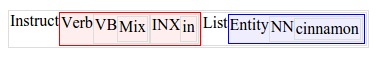
\includegraphics[width=0.9\textwidth]{images/parsing}

\end{frame}

\begin{frame}{Interpreting}
 \begin{itemize}
  \item Interpret Instructions
  \item Save Rule Samples
 \end{itemize}
\end{frame}

\begin{frame}[fragile=singleslide]\frametitle{Interpreting}
 \begin{verbatim}
{
    "index" : 0,
    "name" : "DECLARE",
    "inData" : [],
    "outData" : [ 
        {
            "bicarbonate soda" : {
                "index" : 1,
                "amount" : "2 tsp"
            }
        }
    ],
    "outPointers" : [ 
        "bicarbonate", 
        "soda", 
        "bicarbonate soda"
    ],
    "inPointers" : []
}
 \end{verbatim}
 
\end{frame}

\begin{frame}{Rule Generation}

\begin{itemize}
 \item Apply the a-priori algorithm
 \item Look for frequent sets and confident rules
 \item find ingredients implying an instruction (Forward Rule)
 \item find instructions implying ingredients (Backward Rule)
\end{itemize}



\begin{align}
 \left\{ \text{baking powder}, \text{butter}, \text{+combine}, \text{+cream}, \text{sugar} \right\}
      \rightarrow \text{BAKE} \nonumber \\
  \left\{ \text{eggs}, \text{butter}, \text{+combine}, \text{+cream}, \text{sugar} \right\}
      \rightarrow \text{BAKE} \nonumber 
\end{align}


\end{frame}


\section{Graph Generation}
\begin{frame}{Graph Generation}
\begin{itemize}
 \item Construct a recipe graph back-to-front
 \item Derive previous actions by applying the rules
 \item Terminate when all nodes are satisfied
 \item Trivially satisfy all nodes not satisfiable by rules
 \item Remove nodes randomly (Geom)
\end{itemize}
\end{frame}

\begin{frame}{Graph Postprocessing}
 \begin{itemize}
  \item Remove duplicate subgraphs
  \item Remove unneeded trivial nodes
 \end{itemize}

\end{frame}

\begin{frame}{Graph Evaluation: Scores}
 \begin{itemize}
   \item Violated rules score: \\ Minus points for violated backward rules
   \item Index score: \\ Evaluate the depth of action nodes
   \item Cross ingredience score: \\ Check co-occurrence of ingredients
   \item Downgrade: \\ Punishment for baking without flour
   \item Cross recipe similarity score: \\ Compare with existing recipes
 \end{itemize}

\end{frame}

\section{Results}

\begin{frame}[fragile=singleslide]\frametitle{Example Result}
\begin{verbatim}
 0. Take creamed butter, eggs and sugar
 1. combine
 2. Take blended, stired and sifted vanilla
 3. stir
 4. Take cooked whole milk, cake flour and vanilla extract
 5. combine
 6. Add baking powder and bake
\end{verbatim}
\end{frame}

\begin{frame}[fragile=singleslide]\frametitle{Example Result (Tree)}
\begin{verbatim}
   0: FINALIZE<5.00>()
      1: BAKE<6.50>(u'baking powder',)
         2: COMBINE<8.00>()
            3: STIR<9.00>()
               4: COMBINE<3.75>()
                  5: TRIVIAL(u'butter', u'eggs',
                             u'+cream', u'sugar')
                     4: TRIVIAL(u'+sift', u'vanilla',
                                u'+blend', u'+stir')
            3: TRIVIAL(u'whole milk', u'+cook',
                       u'cake flour', u'vanilla extract')
\end{verbatim}
\end{frame}

\begin{frame}[fragile=singleslide]\frametitle{Example Result (Scores)}
\begin{verbatim}
       Violated rules score: vrs = -0.04
                Index score: ixs = -1.53
    Cross ingredience score: xis =  0.88
           Manual downgrade: mdg =  0.00
NCD Cross recipe similarity: xrd = -0.70
                TOTAL SCORE: SUM = -1.39
\end{verbatim}
\end{frame}

\end{document}
